\documentclass[acmsmall,screen,anonymous]{acmart}
\setcopyright{none}
\settopmatter{printacmref=false}
\usepackage{booktabs}
\usepackage{graphicx}
\begin{document}
\pagestyle{plain}
\begin{center}\large Supporting Results and Analyses\end{center}
This document accompanies the replication package and provides the aggregate and per-task values underlying the result figures, initial-state analyses, and case-level evidence. Pass@1, Secure@1, and Secure-Pass@1 measure passing all hidden functional tests, all hidden security tests, and both, respectively. In candidate-state notation, F and S denote functional and security outcomes; joint repairs and regressions refer to transitions into and out of passing both.
\begin{table}[pos=htbp]
\centering
\caption{Execution feedback with exactly two revisions and 200 paired initial candidates per branch. Fixed selection follows test identifier order. Rates are percentages. Tokens count the two new completions per candidate, excluding the archived initial response.}
\label{tab:supp-fixed-calls}
\begin{tabular}{lrrrr}
\toprule
Branch & Pass@1 & Secure@1 & \textbf{Secure-Pass@1} & Tokens \\
\midrule
Self-review & 59.0 & 67.0 & 50.0 & 407 \\
Binary status & 56.5 & 66.5 & 47.5 & 409 \\
Raw, fixed selection & 56.5 & 69.0 & 51.5 & 416 \\
Raw, security priority & 57.0 & 68.0 & 51.5 & 416 \\
Structured, fixed selection & 59.0 & 70.5 & 53.0 & 437 \\
Structured, security priority & 59.0 & 71.5 & 53.0 & 431 \\
\bottomrule
\end{tabular}
\medskip
\begin{tabular}{lrr}
\toprule
Planned Secure-Pass@1 contrast & Difference (pp) & Holm $p$ \\
\midrule
Binary $-$ self-review & -2.5 & 1.00 \\
Raw (fixed) $-$ binary & 4.0 & 1.00 \\
Security priority $-$ fixed (raw) & 0.0 & 1.00 \\
Structured $-$ raw (fixed) & 1.5 & 1.00 \\
Selection--presentation interaction & 0.0 & 1.00 \\
\bottomrule
\end{tabular}
\end{table}

\begin{table}[t]
\centering
\caption{External project validation: 100 trajectories per method across ten tasks, two models and five seeds. Rates are percentages; calls include the shared initial response as a logical call.}
\label{tab:supp-external-projects}
\begin{tabular}{lrrrr}
\toprule
Method & Pass@1 & Secure@1 & \textbf{Secure-Pass@1} & Calls/candidate \\
\midrule
B0 & 64 & 65 & 32 & 1.00 \\
B3 & 71 & 69 & 42 & 1.00 \\
M  & 60 & 81 & 50 & 2.23 \\
B6 & 70 & 74 & 50 & 2.00 \\
\bottomrule
\end{tabular}
\end{table}

\begin{table}[pos=htbp]
\caption{Project-level pass rates by task (\%), listed as Pass@1 / Secure@1 / Secure-Pass@1 in each cell. Each entry summarizes ten model--seed observations.}
\centering\small
\begin{tabular}{lrrrr}
\toprule
Task & B0 & B3 & M & B6 \\
\midrule
Flask template & 100/0/0 & 70/30/0 & 50/30/0 & 70/30/0 \\
PyYAML & 100/100/100 & 100/100/100 & 100/100/100 & 100/100/100 \\
SQLite3 & 50/100/50 & 70/100/70 & 50/100/50 & 70/100/70 \\
subprocess.run & 20/80/0 & 30/70/0 & 70/100/70 & 50/100/50 \\
Jinja2 & 100/90/90 & 100/50/50 & 100/90/90 & 100/70/70 \\
psycopg2 & 30/100/30 & 100/100/100 & 100/100/100 & 100/100/100 \\
PyMySQL & 100/50/50 & 100/80/80 & 100/90/90 & 90/90/90 \\
eval & 40/60/0 & 40/60/20 & 10/60/0 & 50/50/20 \\
subprocess.Popen & 0/70/0 & 0/100/0 & 0/100/0 & 0/100/0 \\
pickle & 100/0/0 & 100/0/0 & 20/40/0 & 70/0/0 \\
\bottomrule
\end{tabular}
\end{table}

\begin{table}[pos=htbp]
\caption{Representation results by model. Each row contains 60 task--seed observations.}
\centering\small
\begin{tabular}{lllrrr}
\toprule
Model & Content & Expression & Pass@1 (\%) & Secure@1 (\%) & \textbf{Secure-Pass@1} (\%) \\
\midrule
Q2.5-C7B & Functional & Code & 51.7 & 51.7 & 31.7 \\
Q2.5-C7B & Functional & Prose & 38.3 & 40.0 & 21.7 \\
Q2.5-C7B & Functional + security & Code & 55.0 & 63.3 & 38.3 \\
Q2.5-C7B & Functional + security & Prose & 46.7 & 58.3 & 30.0 \\
Q2.5-C14B & Functional & Code & 51.7 & 60.0 & 50.0 \\
Q2.5-C14B & Functional & Prose & 55.0 & 51.7 & 50.0 \\
Q2.5-C14B & Functional + security & Code & 55.0 & 60.0 & 40.0 \\
Q2.5-C14B & Functional + security & Prose & 56.7 & 56.7 & 41.7 \\
\bottomrule
\end{tabular}
\end{table}
\begin{table}[pos=htbp]
\caption{Per-task hidden joint pass rates (\%) for the representation experiment. Each condition has ten model--seed observations per task.}
\centering\small
\begin{tabular}{lrrrr}
\toprule
Task & F/code & F/prose & F+S/code & F+S/prose \\
\midrule
CodeQL\_codeql\_cwe020\_1 & 0 & 0 & 0 & 0 \\
SonarSource\_SS\_cwe079\_0 & 40 & 10 & 30 & 0 \\
SonarSource\_SS\_cwe094\_0 & 60 & 50 & 0 & 0 \\
SonarSource\_SS\_cwe827\_0 & 100 & 100 & 100 & 100 \\
Author\_A\_cwe078\_0 & 60 & 70 & 60 & 70 \\
Author\_A\_cwe089\_1 & 100 & 100 & 100 & 100 \\
CodeQL\_codeql\_cwe079\_0 & 0 & 0 & 0 & 0 \\
StackOverflow\_SO\_cwe094\_4 & 0 & 0 & 50 & 10 \\
cwe-022/0-py & 0 & 0 & 0 & 0 \\
cwe-079/1-py & 80 & 50 & 100 & 100 \\
cwe-117/0-py & 50 & 50 & 30 & 50 \\
cwe-312/0-py & 0 & 0 & 0 & 0 \\
\bottomrule
\end{tabular}
\end{table}

\begin{table}[pos=htbp]
\caption{Security-feedback ablation by model. Each branch has 100 initial candidates per model and exactly two revisions.}
\centering\small
\begin{tabular}{llrrr}
\toprule
Model & Feedback & Pass@1 (\%) & Secure@1 (\%) & \textbf{Secure-Pass@1} (\%) \\
\midrule
Q2.5-C7B & Functional only & 58.0 & 61.0 & 45.0 \\
Q2.5-C7B & Functional + security & 53.0 & 59.0 & 44.0 \\
Q2.5-C14B & Functional only & 68.0 & 69.0 & 58.0 \\
Q2.5-C14B & Functional + security & 68.0 & 74.0 & 63.0 \\
\bottomrule
\end{tabular}
\end{table}
\begin{table}[pos=htbp]
\caption{Security-feedback ablation by task. Each branch has ten model--seed observations per task. Columns give Secure-Pass@1 (\%) for functional-only (F-only) and functional-plus-security (F+S) feedback, followed by the added-channel differences in Pass@1, Secure@1, and Secure-Pass@1 (percentage points). Full rates are in the accompanying CSV.}
\centering\small
\setlength{\tabcolsep}{3pt}
\begin{tabular}{lrrrrr}
\toprule
Task & \shortstack{Secure-Pass@1\\F-only} & \shortstack{Secure-Pass@1\\F+S} & \shortstack{$\Delta$\\Pass@1} & \shortstack{$\Delta$\\Secure@1} & \shortstack{$\Delta$\\Secure-Pass@1} \\
\midrule
CG+/cwe-022/0-py & 0 & 40 & -10 & 50 & 40 \\
CG+/cwe-079/1-py & 90 & 100 & 10 & 0 & 10 \\
CG+/cwe-117/0-py & 0 & 0 & 0 & 0 & 0 \\
CG+/cwe-312/0-py & 0 & 0 & 0 & 0 & 0 \\
CW/cwe\_095\_0 & 40 & 40 & 0 & -10 & 0 \\
CW/cwe\_329\_0 & 60 & 60 & 0 & 0 & 0 \\
CW/cwe\_347\_0 & 100 & 100 & 0 & 0 & 0 \\
CW/cwe\_377\_0 & 100 & 100 & 0 & 0 & 0 \\
CW/cwe\_760\_0 & 100 & 90 & -10 & -10 & -10 \\
CW/cwe\_918\_0 & 50 & 50 & 0 & 0 & 0 \\
CW/cwe\_918\_1 & 40 & 40 & 0 & 0 & 0 \\
CW/cwe\_943\_0 & 100 & 100 & 0 & 0 & 0 \\
SA/CodeQL\_codeql\_cwe020\_1 & 10 & 10 & 0 & 0 & 0 \\
SA/SonarSource\_SS\_cwe079\_0 & 50 & 30 & -20 & -20 & -20 \\
SA/SonarSource\_SS\_cwe094\_0 & 90 & 90 & 0 & 0 & 0 \\
SA/SonarSource\_SS\_cwe827\_0 & 100 & 100 & 0 & 0 & 0 \\
SA/Author\_A\_cwe078\_0 & 0 & 0 & 0 & 0 & 0 \\
SA/Author\_A\_cwe089\_1 & 100 & 100 & 0 & 0 & 0 \\
SA/CodeQL\_codeql\_cwe079\_0 & 0 & 0 & 0 & 0 & 0 \\
SA/StackOverflow\_SO\_cwe094\_4 & 0 & 20 & -20 & 20 & 20 \\
\bottomrule
\end{tabular}
\end{table}
\begin{table}[pos=htbp]
\caption{Initial-to-final hidden states in the security-feedback ablation. Each column contains 200 candidates.}
\centering\small
\begin{tabular}{lrr}
\toprule
Transition & Functional only & Functional + security \\
\midrule
\texttt{F+S+} $\rightarrow$ \texttt{F+S+} & 90 & 89 \\
\texttt{F+S+} $\rightarrow$ \texttt{F-S-} & 0 & 1 \\
\texttt{F+S-} $\rightarrow$ \texttt{F+S+} & 0 & 3 \\
\texttt{F+S-} $\rightarrow$ \texttt{F+S-} & 18 & 13 \\
\texttt{F+S-} $\rightarrow$ \texttt{F-S-} & 0 & 2 \\
\texttt{F-S+} $\rightarrow$ \texttt{F+S+} & 9 & 8 \\
\texttt{F-S+} $\rightarrow$ \texttt{F-S+} & 27 & 25 \\
\texttt{F-S+} $\rightarrow$ \texttt{F-S-} & 4 & 7 \\
\texttt{F-S-} $\rightarrow$ \texttt{F+S+} & 4 & 7 \\
\texttt{F-S-} $\rightarrow$ \texttt{F+S-} & 5 & 1 \\
\texttt{F-S-} $\rightarrow$ \texttt{F-S+} & 0 & 1 \\
\texttt{F-S-} $\rightarrow$ \texttt{F-S-} & 43 & 43 \\
\bottomrule
\end{tabular}
\end{table}
\FloatBarrier
\paragraph{Feedback and generation costs}
Across two revisions, functional-only feedback uses a mean of 1,333.4 prompt tokens, 504.3 completion tokens, and 168.8 delivered feedback tokens per trajectory. Functional-plus-security feedback uses 1,495.5, 517.0, and 270.1 tokens, respectively. Functional channels are truncated in 10 and eight of 400 messages; security channels are truncated in 16 of 400 combined messages. No generation reaches the 3,072-token output cap. Both branches receive the same functional channel at the initial state; subsequent messages reflect their own revised candidates.

\paragraph{Candidate-load failures}
Six visible or hidden evaluations fail during candidate loading. Their responses remain in the grid. Functional feedback reports the visible load error and security feedback reports that tests did not run; final uncollectable candidates fail all three endpoints. The artifact preserves the execution correction, original sources, and generated responses. Hidden results never enter revision messages.

\begin{figure}[t]
\centering
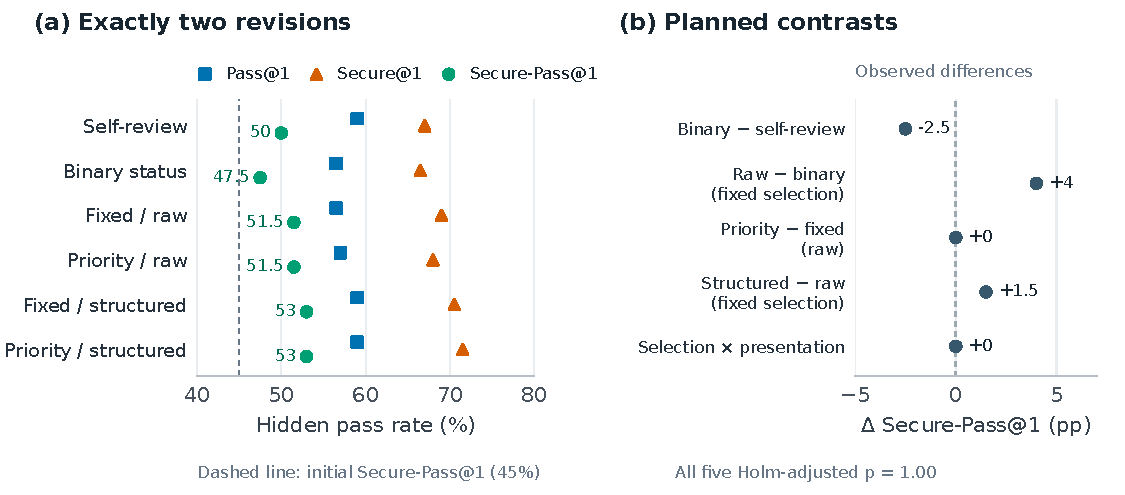
\includegraphics[width=\linewidth]{figures/fixed-call-effects.pdf}
\caption{Fixed two-revision experiment, 200 paired initial candidates per branch. (a) Pass@1, Secure@1, and Secure-Pass@1; the dashed line marks initial Secure-Pass@1 (45\%). (b) Five planned Secure-Pass@1 differences; all Holm-adjusted $p=1$. Observed ties do not establish population equivalence. Complete rates, tokens and contrasts are in the supplementary numeric tables.}
\Description{Left: three metric markers per branch. Right: five effect estimates around a zero reference, with no significant adjusted contrast.}
\label{fig:fixed-calls}
\end{figure}
\begin{table}[pos=htbp]
\caption{Security-feedback outcomes stratified by initial visible state. Final pass rates are Secure-Pass@1 (\%). F-only and F+S denote the two feedback conditions. Each branch makes exactly two revisions. Tasks can occur in multiple strata. F.Reg. counts hidden functional regression relative to the shared initial candidate. These are post-hoc descriptive strata.}
\centering\small
\begin{tabular}{lrrr rrr}
\toprule
Initial visible & Initials & Tasks & \shortstack{Secure-Pass@1\\F-only (\%)} & \shortstack{Secure-Pass@1\\F+S (\%)} & Wins/losses/ties & F.Reg./F+S \\
\midrule
F+S+ & 100 & 12 & 85.0 & 84.0 & 0/1/99 & 1 \\
F+S- & 18 & 4 & 0.0 & 16.7 & 3/0/15 & 2 \\
F-S+ & 50 & 7 & 28.0 & 26.0 & 1/2/47 & 0 \\
F-S- & 32 & 6 & 12.5 & 21.9 & 3/0/29 & 0 \\
\bottomrule
\end{tabular}
\end{table}
\begin{table}[pos=htbp]
\caption{Project-level B0-to-M outcomes by initial visible state. Repair and regression counts use the initial hidden state; a visible functional failure need not imply a hidden functional failure. Calls exclude the shared initial generation.}
\centering\small
\begin{tabular}{lrrrrrr}
\toprule
Initial visible & Initials & Tasks & J repairs & F.Reg. & \shortstack{Secure-Pass@1\\M (\%)} & New calls \\
\midrule
F+S+ & 27 & 6 & 0 & 0 & 85.2 & 0 \\
F+S- & 28 & 7 & 6 & 13 & 21.4 & 47 \\
F-S+ & 39 & 6 & 12 & 0 & 53.8 & 64 \\
F-S- & 6 & 1 & 0 & 3 & 0.0 & 12 \\
\bottomrule
\end{tabular}
\end{table}
\begin{table}[pos=htbp]
\caption{Project-level functional regression mechanisms. Categories describe the observed execution failures in all 16 B0-to-M regressions.}
\centering\small
\begin{tabular}{lrl}
\toprule
Mechanism & Count & Cases \\
\midrule
Response extraction / loading failure & 6 & EX02, EX08, EX10--11, EX15--16 \\
Unpickler used as context manager & 4 & EX04--07 \\
Template syntax or interpolation damage & 3 & EX12--14 \\
AST interpreter semantic errors & 2 & EX01, EX03 \\
Overrestrictive preference schema & 1 & EX09 \\
\bottomrule
\end{tabular}
\end{table}
\FloatBarrier
\paragraph{Case selection and evidence}
The artifact ledger includes all ten security-feedback joint disagreements, plus two additional functional regressions that tie on joint failure, and all 16 project-level B0-to-M functional regressions. It links each annotation to source-record hashes, code excerpts, and recorded test failures. Case classifications use machine-assisted source/log inspection. Automated checks verify completeness of case selection and correspondence between annotations and archived evidence. The analysis uses the archived generations and original outcome scores.

\paragraph{Security-feedback cases}
SF01--04 add a null-result guard after \texttt{safe\_join} to handle an exception on rejected traversal input. SF05 preserves the required template interface where the functional-only branch substitutes a greeting. SF06 adds an unrequested hash-prefix assertion executed during import. SF07--08 use \texttt{escape} without an import. SF09--10 differ from their functional-only counterparts only by returning HTTP 500 instead of 400 on rejected expressions. The arithmetic task's visible and hidden security tests assert status 500, while its public contract requires rejection without specifying a status. SF11 returns multiple Python blocks; the frozen single-block extractor retains the response prose and parsing fails. SF12 introduces unavailable \texttt{sympy}. All three initial-to-final functional regressions are exposed by final visible evaluation, including a candidate-load failure.

\paragraph{Project-level regressions}
EX01 resolves \texttt{input\_data} as a dictionary key instead of the variable binding; EX03 rejects string subscripts. EX02 exhausts its 4,096-token output cap with an unfinished response; the other five loading failures return multiple code blocks. EX04--07 raise a context-manager \texttt{TypeError} before unpickling benign or malicious data. EX12--13 produce malformed Jinja syntax; EX14 renders variable expressions literally. Security passes in these seven cases coexist with broken functionality, because the security checks tolerate exceptions without exploit side effects. EX09 restricts preferences to \texttt{theme}/\texttt{language}, rejecting the legitimate hidden \texttt{notifications} key; its visible functional example contains only the two allowed keys. Validation after \texttt{pickle.loads} also fails to prevent recorded malicious side effects.

Fifteen of the 16 regressions fail the final visible functional test and remain unresolved at the revision limit. EX09 passes the visible test but fails on a legitimate hidden input. The cases therefore distinguish incomplete repair of exposed failures from a gap in visible test coverage.

\paragraph{Opportunity, costs, and sensitivity}
Initial-state strata retain all 200 paired initials and all 100 project-level B0 initials. No stratum uses revised code or hidden outcomes for assignment. The accompanying CSV gives Pass@1, Secure@1, Secure-Pass@1, repairs, regressions, calls, and mean input/output tokens for each stratum; JSON additionally retains model breakdowns for the security-feedback experiment. The whole-task sensitivity analysis excludes all ten arithmetic-task pairs: functional-only and combined feedback score 54.21\% and 55.26\% joint success on the remaining 190 pairs. This post-hoc sensitivity analysis accompanies the full 20-task results.

\begin{table}[t]
\caption{Paired feedback transitions over shared initial candidates. Task--rep. cells are repeated observations, not independent inference units. Repair denotes hidden joint failure $\rightarrow$ success; Trig. denotes at least one revision; J.Reg./F.Reg. denote hidden joint/function regression; Sec.-only denotes $F^+S^-\rightarrow F^+S^+$.}
\label{tab:feedback}
\centering
\begin{tabular}{lrrrrrr}
\toprule
Comparison & Task--rep. & Trig. & Repair & J.Reg. & F.Reg. & Sec.-only \\
\midrule
B4 $-$ B0 & 465 & 252 & 83 & 3 & 15 & 45 \\
M $-$ B0 & 465 & 252 & 80 & 0 & 8 & 40 \\
B6 $-$ B3 & 330 & 47 & 18 & 0 & 0 & 2 \\
M $-$ B4 & 465 & 252 & 6 & 6 & 8 & 0 \\
\bottomrule
\end{tabular}

\end{table}
\end{document}
